\section{Experiment}


As stated before, we want to investigate at what rotational (horizontal) gains does the user notice that the virtual world and the real world rotations are different? With the subresearch question is this number different when people are engaged in a task versus when a person is just walking around without specific tasks?\\
\\
This subject has already been investigated by other rechears \cite{steinicke2}. The reliability of this experiment could be doubted however, because this experiment involved a small group of testpersons and therefore some conclusions could be made which were in fact not true if you had a larger and thus more reliable test group. Though we are als not able to do experiments with a large group we still want to (re)do the experiment and see if we have results which are in accordance with the results Steiniche had.

\subsection{Detailed description of the desired experiment}\label{sec:description}
At first we designed an experiment which was like the one Steinicke conducted. We would conduct two experiments, one with a group of people which will not conduct a specific task during the experiment and one with a group of people who are engaged in a task during the experiment. Lets call the first experiment, experiment A and the second experiment B. Both experiments are executed multiple times with a single person per time per experiment. First we shall describe experiment A.\\
In this experiment a single person would wear an Oculus Rift. With this Oculus that person could see a virtual world. This is a very simple empty room with on the floor a twisting path. The test person is asked to walk over that path in the virtual world until they can walk no further. The test person will walk through this room a couple of times. Each time we will change the rotational gain a bit, but the user does not know this. Afterwards we will ask the testperson some questions. Did they noticed something strange in the virtual world during the experiment and if so what was it? Next a little more specific did they notice something about the rotational gains? Were these higher or lower than in the real world? After they answered these questions they are finished with the experiment. During the experiment we will have rotational gains between the 0,5 and the 1,5. This means if the gain is 0,5 a person turns with half the speed in the virtual world as they would in the real and the gain of 1,5 means that a person would turn 1,5 times as fast in the virtual world as in the real world. Of course if the gain in 1, this simply means that there is no difference. \\
Now lets describe experiment B. The people in this test case do exactly the same as all the people in experiment A only while walking on the path in the virtual world a couloured dot/circle is shown in front of them and they are asked to raise their hand when this dot changes colors. The goal is of course to distract them from the route. \\
A very important thing to mention is that  if a person participates in experiment A, he or she cannot participate in experiment B, because they overlap so much. During the experiment we will use the motion track function of the Oculus Rift to track the route the testpersons are walking.

\subsection{Relation between Experiment and Research Question and potentional problems}\label{sec:rel}
The people that will participate in our experiment follow the course \emph{Interactive Virtual Environments}.
This means they know at least something about redirected walking.
This could influence their ability to perceive differences in the gains.
Since this would influence both groups, we assume both groups are effected equally.
This means that we can still compare the test group with the control group.

Our groups will consist mostly of students.
This means that we won't have a lot of diversity in age.
This could influence their ability to perceive differences in the gains, because elder or younger people could be better or worse in perceiving the gains.
Since this would influence both groups, we assume both groups are effected equally.
This means that we can still compare the test group with the control group.

We do not have enough people who are willing to do the experiment.
This means that the results are not really reliable.
We are trying to make this up with letting the users do the experiment multiple times, however this could influence the results.
The control group could get bored and not focus at all and the task for the test group could be not engaging enough the next times, which means they have more time to focus.

We miss a method to compare the perceived gains for each user.
We are now limited to the answers of the questions of each user.
How each user perceives and answers these question, can be different.
Other methods could be asking the users how they think that they have walked and compare it with the path they walked in the virtual environment.
However also this method is limited, because it is hard to grade how good or bad he perceived the gains.

\subsection{Bottlenecks in the experiment design and eventual experiment}
When we started testing with the Oculus Rift we encoutered several problems, these problems meant that we had to alter our experiment on a couple of points, because otherwise it could not be conducted. The first problem was the motion tracking. We used a development kit 2 to work with the rift and it was stated that this kit had motion tracking, but in reality this motion tracking was so bad it could track a few steps to the side and only one or two steps to the front and back. This means that this was usable for a gaming console like the Wii where a person stands on a single place and only turns its body a bit, but for tracking a route a person is walking this was totally useless. We tried to fix this by using bluetooth triangulation with our cellphones. This means we would place our phones in the corners of the physical room and they send sighnals to the Oculus so we could measure where it was. In theory this was a good solution but in pratical this was way too slow to use it. At this point we gave up the tracking and we used another solution for "walking". We gave the test person a Playstation 3 controller which only allows participants to move in the direction they are facing.
The test subject stands in a spot and moves forward in the virtual world using the controller.
When the path reaches a bend, the gyroscopic sensors of the Oculus Rift are to be used to rotate in the virtual world.
We had the test subjects rotate their entire body, instead of just the head, as turning just the head might give away the gains used, due to straining of the neck.
Additionally, when walking in real life, changing direction is mostly done with the entire body as well.\\
\begin{figure}[htb]
	\centering
	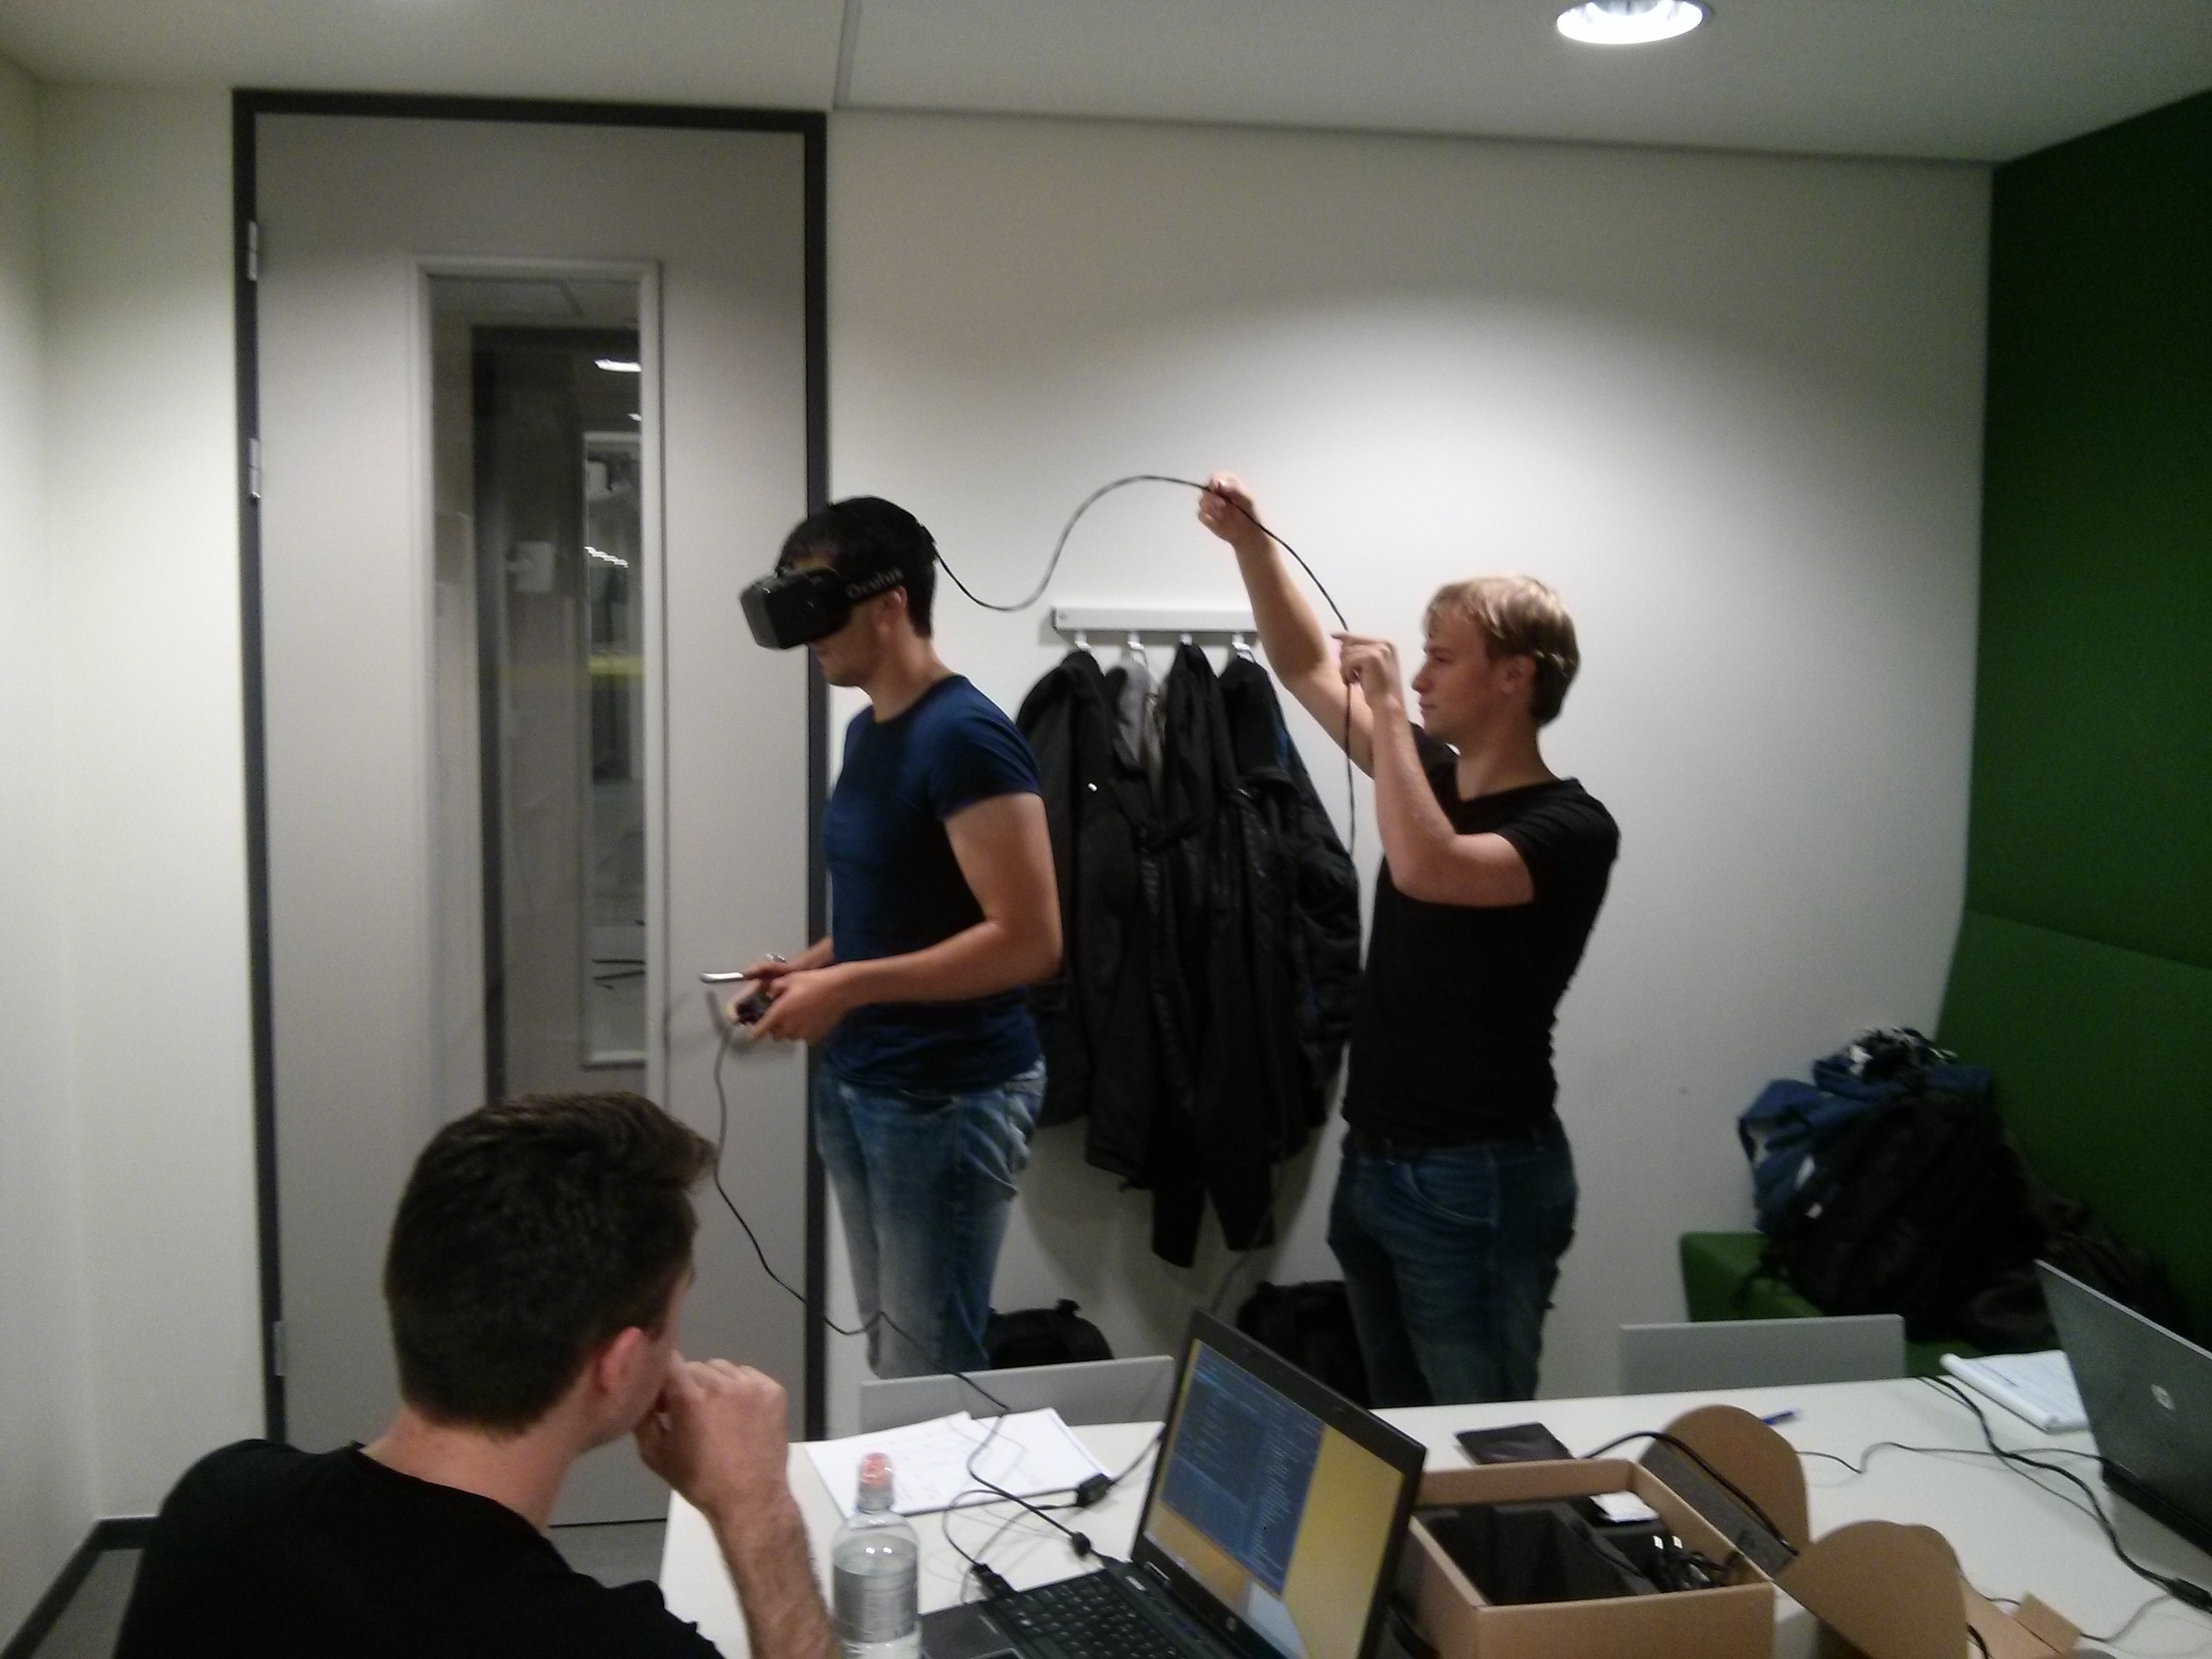
\includegraphics[width=\linewidth]{sections/finalreport/images/experiment.jpg}	
	\caption{A picture of the eventual experiment}
\end{figure}
\\ \\ 
The next problem we had was a lack of time to test with the Oculus Rift. We were only allowed to use the Oculus two hours a week. Unfortunately we wasted one of these sessions on a broken Oculus and one on fixing the tracking problem. As a result we had not a lot of time left to do the actual experiment and inplement the color changing dot. This made the implementation of the dot unfeasible. Therefore we chose a more practical and perhaps even more effective method to distract the test subjects from focusing on the path too much, we gave the test subjects simple (arithmetic) calculations to solve.
This simultaneously serves as the previously planned task in which we engage test subjects.\\
\\
Another bottleneck in our original experiment was the fact that we would ask the questions after multiple runs.This could result that the test subject could mix up test runs. On the other hand, asking the questions after every single test run may cause the test subject to be biased when doing the next run.
Therefore, we let each test subject only do the experiment once and not multiple times.
As a result, however, we did not manage to gather a lot of data, but we did manage to analyze this data and find some similarities or some peculiarities.

\subsection{Software Implementation}
\subsubsection{Requirements}
As for software implementation, we defined several objectives.
First of all, we have to produce a virtual environment, in which we can place the test subjects.
This virtual environment should include a path on which the user is to walk, which should contain bends, such that the user is forced to rotate in order to traverse it.
Accordingly, the software should read the input from the Oculus Rift, allowing real-world head movements to be translated to virtual world rotations.
Apart from rotating, the test subject should also be able to move around in the virtual environment. 
Furthermore, the software should contain a manners of having the test subject do additional tasks, such that we can split the test subjects into two groups: one having to do an extra task, and a control group, such that we can see if mentally engaging task influence the results.\\
Additionally, the ones conducting the experiment should be able to easily adjust the rotational gains discussed in previous sections.
Since every test subject is tested with but a single rotational gain, the adjustments to not have to be performed on the fly, but might be done in between experiments, when the next subject is instructed on the experiment.

\subsubsection{Implementation challenges}
Some of these requirements could be met rather easily, but seemed to make other requirements more difficult to achieve.
Along with the drivers and utility software of the Oculus Rift, we downloaded the Oculus SDK, the software development kit.
Initially, we had planned on having to make the virtual environment ourselves.
This would be possible, as we have had some experience in both software development and visualization, but it would still cost a substantial amount of time.
Since experiments had to be conducted as well, this would prove unfeasible in the time span during which the project had to be completed.
Luckily, the SDK came with executable code examples, which both allowed us test the Oculus Rift, and served as a base project for us to make adjustments to. \\
However, using given code does come with consequences.
Before getting to alter the code, we must first understand the code given to us.
The projects actually contained quite a lot of code, so understanding the code and determining which parts are interesting to us is a rather lengthy process.
Moreover, as it turned out, access to the underlying Oculus code was limited to a large extent. \\

Ideally, we would have edited the code that read input from the Oculus Rift, and adjust the degrees of rotation read according to the rotational gain that was set, however, the Oculus SDK does not allow altering of code at that level.
Using example code instead of writing our own code actually made it rather difficult to implement rotational gains.
Instead, we had to be a little more creative to achieve the desired effect.
It forced us to find functions which we can alter, such that rotational gains can be achieved, without breaking the intended effect of the function.
This is a rather dangerous method, as it is hard to tell when and where already implemented functions will be used.
However, we managed to find several possible solutions. \\

First of all, and perhaps the most simple solution, was to recalibrate the Oculus Rift.
The Oculus Rift is calibrated, such that every degree it turns in the real world corresponds to a degree of rotation in the virtual world.
If we could somehow calibrate it `wrongly', such that every degree in the real world would correspond to the rotational gain, we would not have to adjust the code at all.
However, this solution does come with risks.
First of all, there is the possibility that something goes wrong in the calibration process.
This might render the Oculus Rift unusable, which would not only be detrimental to ourselves, but to other groups using it as well.
Moreover, the Oculus Rift we used was borrowed from the Fontys college, so had to be treated with care.
Additionally, it would be quite the hassle to have to recalibrate the Oculus Rift for each test subject.
Therefore, we decided that this solution was unsuitable.\\

During the process of trying to understand the given code, we found that the rate at which the virtual rotation was adjusted, was dependent on the frame rate of the demo program.
The frame rate of games and visualization programs is usually set to a constant frame rate, which the computer attempts to meet during execution.
Indeed we found that in the code, the frame rate was set at 60 frames per second (FPS).
We figured that if we could adjust the frame rate of the program, the rotation rate would change as well, resulting in rotational gains if the FPS is set to a higher amount.
The correlation is linear, i.e. if we were to set the frame rate to 90 FPS, instead of 60, the resulting gain would be $1.5$.
This method would allow us to change the rotational gain, simply by editing a single value in the code.
In contrast to the previously suggested method, this can be done very quickly in between test subjects.
However, this method has certain disadvantages as well. \\
Increasing the frame rate also increases the computational load of the program.
While the computer was able to maintain a frame rate of 60 FPS without too many problems, increasing it might become heavy a load for the computer.
A possible outcome would be that the computer cannot maintain a given frame rate, and thus the rotational gains would not be constant, which would make the test results inaccurate. \\
Then again, even if the computer would be able to render the program at a higher frame rate, the frame rate itself might influence the results.
In our experiment, we test both positive and negative rotational gains.
To achieve negative rotational gains, the frame rate would have to be lowered.
However, the user would notice a drop in frame rate.
A lower frame rate would result in a less smooth image, which might affect the level of immersion in the program.
Since we want our results to be dependent solely on the rotational gains, this method would not suit our needs either. \\

Finally, we noticed the the program accepted mouse input.
As the mouse moves, its location, relative to its previous location, is saved to a variable.
Then, every frame, this relative location is translated to a rotation in the virtual world, and the relative location is reset.
The extra mouse rotation is calculated separately from the Oculus Rift input.
Since we want users to rotate solely using the Oculus Rift, the mouse rotation is left unused, and can be used by us to add gains instead. \\
Though our access to the underlying Oculus code was limited, there was in fact a function to read the current Oculus rotation, which could be used to our advantage.
In the altered code, we save the current rotation of the Oculus, and calculate the difference with the previous rotation every frame.
This then corresponds to the actual rotation change that was made in every frame.
We can then multiply this by the rotational gains we are trying to achieve, and then interpret this as mouse movement. \\
Let $r$ denote the rotational gain, $d$ denote the difference in angle of the Oculus Rift between two frames, and $m$ the exported mouse output. 
Say that normal rotation, without any alterations has a rotational gains value of $r = 1$, as defined by the paper we have studied.
We can then compute the exported mouse output as: $m = d(r - 1)$.
In this way, we are able to have both negative and positive rotational gains, or no gains at all. \\
There are several advantages to this method.
Firstly, it allows the rotational gains to be quickly and easily adapted between test subjects, as it is a single constant in the program.
Additionally, in contrast with adjusting the frame rate, this method does not introduce any kind of inaccuracy to the test results, nor are there any significant effects on the computational power required.
Moreover, it was rather easily implemented, when we had studied the code sufficiently. \\

After implementing the solution mentioned above, we went ahead and tested it ourselves.
Whilst the solution did seem to work, we noticed that it also introduced a bug to the system.
We noticed that with high positive gains, the virtual world seemed to jump in rotation, where the user would suddenly face in a different direction.
This occurred when the user would rotate a certain number of degrees from the center, and occurred at either sides.
After testing, we concluded that where this jump occurred was indeed correlated to the positive gain that was set. 
With a gain of 1, i.e. natural rotation, there was no jump.
At gains higher than one, the jump would occur between the initial rotation and half a circle, closing in on the initial rotation the higher the gain got.
At gains lower than one, the jump would occur when spinning over half a circle, going further away as the gain decreased. \\
Since we had had some problems with the Oculus Rift before, we faced an imminent shortage of time, and had to get started with testing as soon as possible.
As a result, we were not able to locate and solve the bug completely, but came up with a temporary solution.
In between test subjects, a member of our team would put on the Oculus Rift, and attempt to find the jump in rotation.
Using the mouse, we could then rotate the virtual world to a point such that it was farthest away from the jump in both directions.
Luckily, with the gains that we used with the experiment and the path that we made, normal traversal of the path would not result in the test subject experiencing the jump.
However, as explained above, we have tested with even higher rotational gains, which would reduce the rotational freedom without finding the jump.
At gains high enough, for example 2 or higher, path traversal would become increasingly difficult, to a point in which it was not possible at all. \\
Even though we had to give up on solving the bug, in retrospect, we do have an idea on what may have caused it.
As previously explained, we were able to read the current rotation from the Oculus Rift.
What we had not checked, was how the altered data was saved and used. 
Instead of saving absolute rotation, the code may save values between 0 and 360 degrees. 
As the user would turn around, especially with higher rotational gains, the 360 degrees may be reached much sooner.
The headset might then jump from 360 back to 1 degrees, instead of going to 361 degrees of rotation. 
The code as is would interpret this as a change in rotation of 359 degrees, which may indeed cause a jump.
This does correspond to what we have seen in testing, where higher rotational gains make the virtual world jump sooner, since the edges of the rotation would then be reached sooner, and vice versa for lower rotational gains. \\
The bug may be solved by changing the difference calculation.
After the first calculation is complete, we could take the result, and subtract it with 360, and then pick the lowest of both absolute values.
This would work in most cases, as it is unlikely that a user would spin over 180 degrees in the time span of a single frame, which is mostly $\frac{1}{60}$ seconds.
However, since we no longer have an Oculus Rift, we will not be able to test this. \\

Some of the requirements were actually made much easier to achieve by using the code provided by the SDK.
As mentioned earlier, the SDK provided us with an executable demo world. 
This code already included input for the Oculus Rift, mouse input, collision detection, and an actual world with walls and a floor.
In fact, we could quite easily find the piece of code responsible for creating walls, and adapted it, to create a path instead.
Walls are creating by providing underlying code with a set of vertices - points in 3d space.
Creating a path was as simple as adding a list of vertices a tad lower to the ground.

\subsubsection{Changes in Requirements}
Some of the requirements specified turned out to be unfeasible in the given amount of time.
Initially, the experiment was designed to have the test subjects walk around in real life as well.
However, tracking seemed to be rather difficult. 
The Oculus Rift DK2 does come with a movement tracker, but it was not efficient enough for large scale tracking.
We then played with the idea to track a test subject using bluetooth, but this turned out to be too slow.
Eventually, we settled with not having the test subjects move at all, and instead let them move around in the virtual world using a joystick. \\
We had access to a Playstation 3 controller to serve as joystick, however, these are not natively supported by the windows operating system.
Luckily, there is a multitude of tools online that allow the controller to communicate with the computer, both through cable and via bluetooth.
Specifically, we relied upon a tool called \textit{MotioninJoy}.
This not only allowed us to use the controller with windows, but also allowed us to remap the controls to specific keys or macros in windows.
Counterintuitively, we actually had to restrict the test subjects in their movement.
The software should only allow the test subjects to move forward, as allowing the test subjects to move in other directions, would allow them to traverse the path without rotating, which is key in this experiment.
To solve this, we used the MotioninJoy tool to map only the forward controls to the letter `w' on the keyboard. 
In the demo program, keyboard keys are already mapped to movements in the virtual environment, where `w' corresponds to forward motion.
This allowed us to use the controller to have the user move in the virtual world efficiently. \\

Secondly, we had planned to have some test subjects perform some mentally engaging task, to see whether this had any effect on the experiment.
We planned on doing so by placing a sphere in the virtual environment, and have the test subject raise his hand when the colour changes.
Again, using predefined code made this exponentially harder.
While we may have been able to create a sphere in the world, doing so would take some rather invasive action in the code, which may have caused failure.
In contradiction to the walls, it was not as simple as simply putting in a list of vectors.
Moreover, having it change colour would be harder still, requiring much more code.
Additionally, we would have to create methods to have it change somewhat randomly, as a regular change of colour would not be enough to keep the test subject sufficiently engaged.
This was not possible in the time we had to our disposal. \\
In the end, a more easy, and perhaps even more efficient means of meeting this requirement, was to simply have the test subject solve simple arithmetic calculations.